\subsection{Development View}

\subsubsection{Package Diagram}

The following package diagram presents the modular decomposition of the F-LOW system. It illustrates how the system is organized into high-level packages, each encapsulating a major responsibility within the architecture.

\begin{figure}[H]
    \centering
    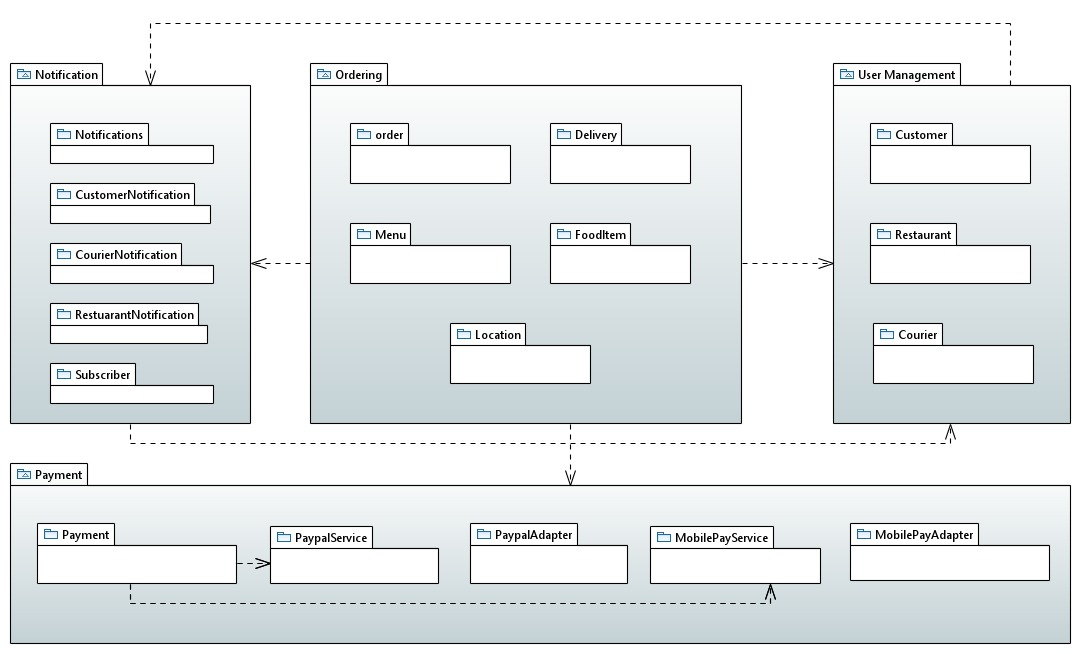
\includegraphics[width=0.9\textwidth]{FIGS/PackageDiagram.jpg}
    \caption{Package Diagram of the F-LOW System}
\end{figure}

Each package encapsulates a specific aspect of the system:

\begin{enumerate}
    \item \textbf{User Management}: Manages user entities such as \texttt{Customer}, \texttt{Courier}, and \texttt{Restaurant}. These entities serve as primary actors throughout the system.
    \item \textbf{Ordering}: Handles business logic for placing, updating, and tracking orders. It integrates food items, menus, delivery logistics, and location services.
    \item \textbf{Payment}: Defines the abstract interface for handling transactions. It supports adapters for multiple services (e.g., PayPal, MobilePay) via the Adapter pattern.
    \item \textbf{Notification}: Implements an event-based architecture using the Observer pattern. It sends updates to users based on state changes in ordering or delivery.
\end{enumerate}

\paragraph{\textbf{\texttt{<<import>>}} Dependencies:}The following relationships are modeled using the \texttt{<<import>>} stereotype to indicate a strong dependency at the interface level:\\
\textbf{Ordering $\rightarrow$ User Management}: Order components directly reference entities such as \texttt{Customer}, \texttt{Courier}, and \texttt{Restaurant} to bind orders to users.\\
\textbf{Ordering $\rightarrow$ Payment}: The \texttt{Order} logic calls the \texttt{pay(info, provider)} method provided by the \texttt{Payment} interface.\\
\textbf{User Management $\rightarrow$ Notification}: Actors like \texttt{Customer}, \texttt{Restaurant}, and \texttt{Courier} subscribe to notification events for receiving system updates.\\
\textbf{Ordering $\rightarrow$ Notification}: Classes such as \texttt{Order} and \texttt{Delivery} generate notifications, relying on \texttt{Notification} and \texttt{Subscriber} components.

\paragraph{Plain Dependencies:}Dashed arrows without stereotypes indicate looser coupling where only selected types are referenced without full namespace import:\\
\textbf{Payment $\dashrightarrow$ PaypalService / MobilePayService}: These services are specific implementations used internally by their respective adapters; they are not exposed system-wide.\\
\textbf{Notification $\dashrightarrow$ User Management}: Notification components may reference actor instances to deliver updates, but do not rely on their full interfaces or APIs.

This separation of concerns through modular packaging ensures extensibility, minimizes coupling, and enables cohesive subsystem development aligned with sound architectural principles.

\subsubsection{Component Diagram}

\begin{figure}[H]
    \centering
    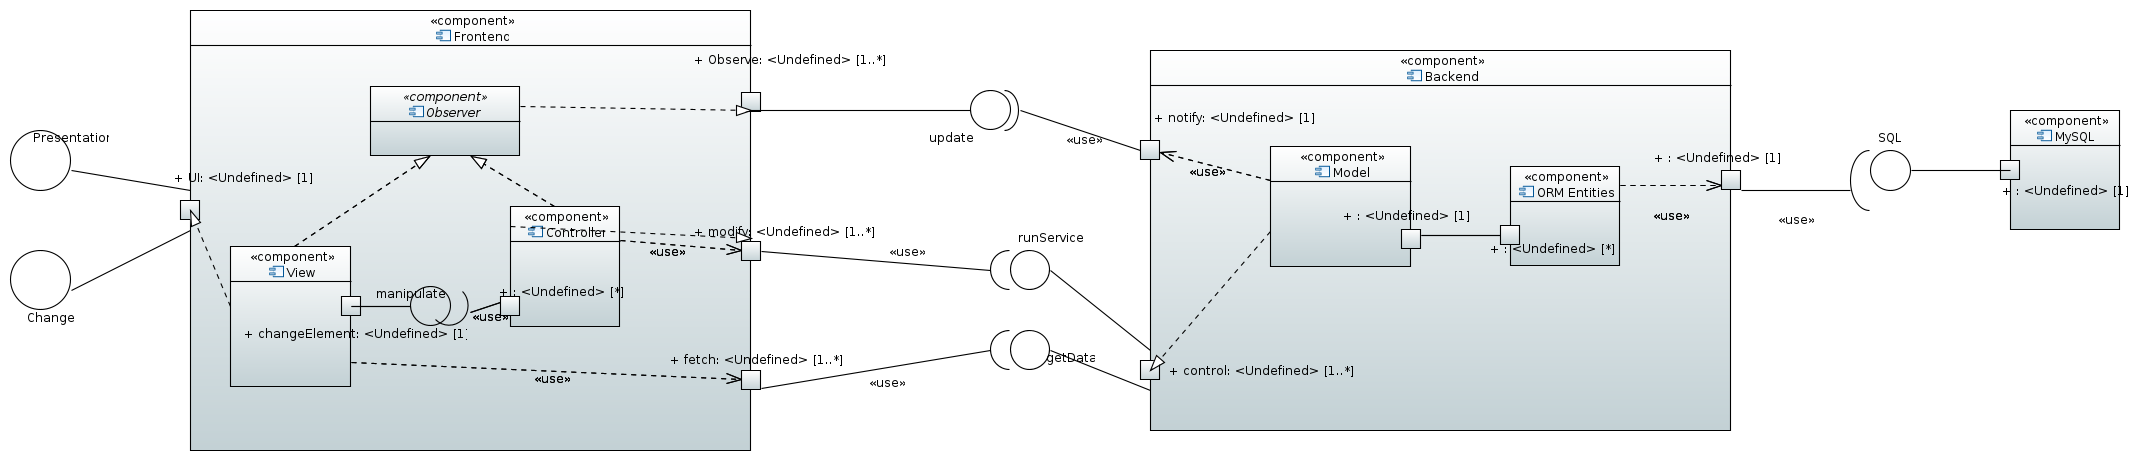
\includegraphics[width=0.9\textwidth]{FIGS/Subsystems.PNG}
    \caption{Component Diagram for the Subsystems in the System}
\end{figure}

As described in the UML standard, the highest-level components of the system are usually called the subsystems. This way, Figure 6 provides a component diagram for the subsystems of our application. The two most important components of our application are, similar to many other web applications, Frontend and Backend. Frontend is responsible for interacting with the user input. In other words, it stands on the client side and communicates with the server according to user input. Most of the server logic is implemented in the Backend Component.

As it is clear in the process view of this architecture document (more specifically, the sequence diagrams), we adopted an MVC architecture pattern in throughout our development process. Therefore, we needed to combine MVC with a popular Frontend-Backend architecture style. As a result, we decided to make the frontend component the observer for our model (business logic), which is implemented by the backend.

Exploring the final result, we see that View components reside within the frontend, responsible for presenting the suitable UI elements to the user. These views are passively fetching data from the backend and showing them with the right format to the user.
In parallel, there are different controllers built into the view components that are listening for user inputs and trigger services on the model side of the application. All in all, runService (required by the controllers) and getData (required mostly by the views) would be the interfaces that Backend provides for Frontend. It is worth noting that all these communications from the client side to the server side can be simply implemented using the HTTP protocol.

On the other hand, Model requires some interface for notifying the observers that they should update according to the fresh data. This is necessary as the user's interactions may result in data transformation on the server. As a result, all the observers (either controllers or views) provide an update interface, which is required by the models. Worthwile to note that this part of the communication from the server-side to the client-side is implemented using the WebSocket protocol.